\chapter{Endgames: Perfect Situation in~Perfect-Information Games}

For many games, solving their late stages (so-called \emph{endgames}) can be done in~an~online way.
In other words, we are often able to postpone the computation of~the endgame strategy until the endgame itself is reached in~the play.

This is especially the case of~perfect-information games such as chess or Go, where the endgame technique has been used for long time.
In these domains, online endgame solving has~significant importance, as it substantially improves the playing quality of~agents.

\section{Chess Endgames}
\todo

\section{Go Endgames}
\todo

\subsection{Why Focus on Go Endgames?}

Martin~\Mueller (in~his dissertation~\cite{Muller1995computer}) mentions the following advantages of~Go endgames for research:
\begin{itemize}
  \item The complexity of~the game often decreases towards the end.
    This allows the study of~Go in a~controlled, simplified context.
  \item An~exact solution is possible for some classes of~endgame positions.
  \item The exact solution of~parts of~a~Go board facilitates the analysis of the rest.
    Reaching the ultimate goal of~winning the game is easier when complete information about part of~the game is at~hand.
    Such information is useful as~additional input for the heuristics that deal with the rest of~the board.

    Human experts use similar reasoning: they observe the score continually from the early midgame, and base their strategic decisions on~such an~analysis (\cite{Takagawa85}).
  \item Some methods developed for partitioning, searching and scoring during endgame carry over to the midgame and opening.
    As programs improve, fewer game-deciding blunders will occur, so the importance of~endgame-type calculation is bound to~increase.
  \item On~a~more philosophical note, the endgame relates to the full game of~Go similarly as Go relates to~real world AI problems.
    It provides a~simplified, more controlled sub-domain that allows the use of~stronger theoretical models than the larger, more general problem.
\end{itemize}

\subsection{Partitioning an~Endgame into Local (Sub)games}

According to~(\cite{Muller1995computer}), there are very strong reasons to~partition board positions during endgames in~Go:
\begin{quotation}
  A~Go position usually consists of~several local scenes that can be analyzed individually.
  In the opening, these scenes can be far apart, and their influence on~each other may be weak.
  A~better partition occurs late in the game, when there are walls of~stones dividing the board.
  A~move cannot have any influence across a~wall of~safe stones.

  \begin{figure}[H]
    \centering
    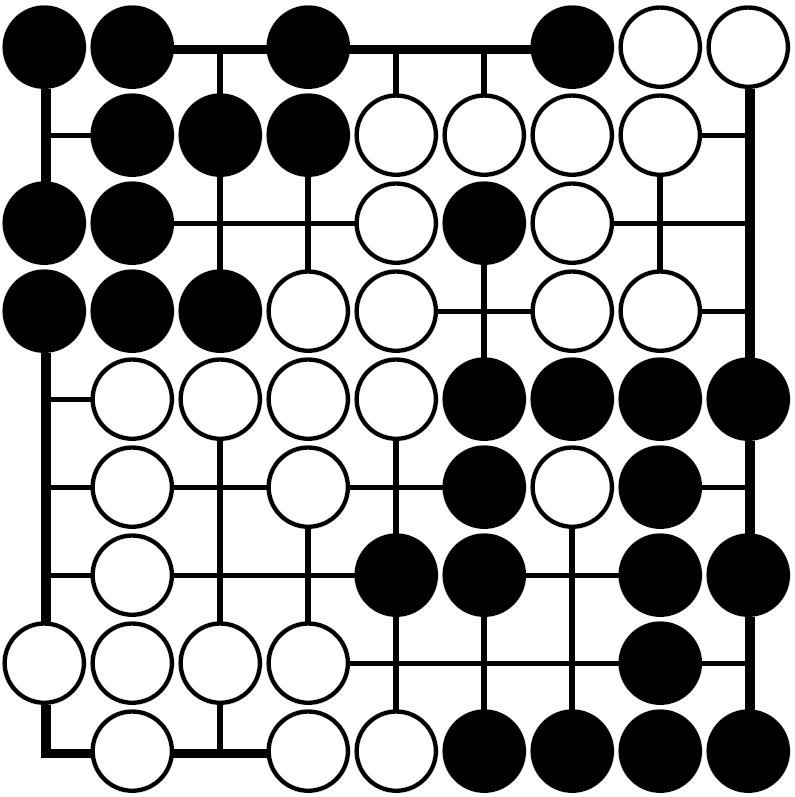
\includegraphics[width=.4\textwidth]{../img/late_endgame_Go_position_suited_for_exact_analysis.png}
    \caption{Late endgame position suited for exact analysis}
    \label{fig:late-Go-endgame}
  \end{figure}

  Board partition improves when many safe walls are on~the board.
  In the opening and midgame, any partition can be approximate at best.
  In the endgame, the partition gets more precise when the status of~all big groups has been settled, and the outlines of~territories are clear.
  When stones become ``immortal'', significant parts of~the board definitely belong to one of the players.
  The connected components of~the rest of~the board form local games that are independent from each other.

  If each local game is simple enough to~analyze completely (such as in Figure~\ref{fig:late-Go-endgame}), combinatorial game theory can compute an~optimal move for the full board position.
\end{quotation}

\subsection{Playing Computer Go as a~Sum of~Local Games}

This is the general procedure for playing Go as a~sum of~local games used in~(\cite{Muller1995computer}):
\begin{enumerate}
  \item Board partition: find safe blocks, safe territories, and local areas.
  \item Generate local game trees in each area.
  \item Evaluate local terminal positions.
  \item Transform local game trees into mathematical games (and simplify games).
  \item Find an optimal move in the sum game and play it.
\end{enumerate}
\Mueller proposes heuristic algorithms for playing the entire game, and exact algorithms for late endgame positions.
Thus, the task of~solving endgames in 1995---at the age of Computer Go's infancy---already played a~vital role.

\subsection{AlphaGo}
\todo
